%===============================================================================
% LaTeX sjabloon voor de bachelorproef toegepaste informatica aan HOGENT
% Meer info op https://github.com/HoGentTIN/latex-hogent-report
%===============================================================================

\documentclass[dutch,dit,thesis]{hogentreport}

% TODO:
% - If necessary, replace the option `dit`' with your own department!
%   Valid entries are dbo, dbt, dgz, dit, dlo, dog, dsa, soa
% - If you write your thesis in English (remark: only possible after getting
%   explicit approval!), remove the option "dutch," or replace with "english".

\usepackage{lipsum} % For blind text, can be removed after adding actual content

%% Pictures to include in the text can be put in the graphics/ folder
\graphicspath{{graphics/}}

%% For source code highlighting, requires pygments to be installed
%% Compile with the -shell-escape flag!
\usepackage[section]{minted}
\usemintedstyle{solarized-light}
\definecolor{bg}{RGB}{253,246,227} %% Set the background color of the codeframe

%% Change this line to edit the line numbering style:
\renewcommand{\theFancyVerbLine}{\ttfamily\scriptsize\arabic{FancyVerbLine}}

%% Macro definition to load external java source files with \javacode{filename}:
\newmintedfile[javacode]{java}{
    bgcolor=bg,
    fontfamily=tt,
    linenos=true,
    numberblanklines=true,
    numbersep=5pt,
    gobble=0,
    framesep=2mm,
    funcnamehighlighting=true,
    tabsize=4,
    obeytabs=false,
    breaklines=true,
    mathescape=false
    samepage=false,
    showspaces=false,
    showtabs =false,
    texcl=false,
}

% Other packages not already included can be imported here
\usepackage{listings}
\usepackage{color}

\definecolor{dkgreen}{rgb}{0,0.6,0}
\definecolor{gray}{rgb}{0.5,0.5,0.5}
\definecolor{mauve}{rgb}{0.58,0,0.82}

\lstset{frame=tb,
    language=java,
    aboveskip=3mm,
    belowskip=3mm,
    showstringspaces=false,
    columns=flexible,
    basicstyle={\small\ttfamily},
    numbers=none,
    numberstyle=\tiny\color{gray},
    keywordstyle=\color{blue},
    commentstyle=\color{dkgreen},
    stringstyle=\color{mauve},
    breaklines=true,
    breakatwhitespace=true,
    tabsize=3
}

%%---------- Document metadata -------------------------------------------------
% TODO: Replace this with your own information
\author{Bram Stevens}
\supervisor{Dhr. J. Willem}
\cosupervisor{Dhr. S. Dedeken}
\title[]%
    {Implementatie van GraphQL binnen een
        zelfontwikkelde accelerator}
\academicyear{\advance\year by 0 \the\year--\advance\year by 1 \the\year}
\examperiod{1}
\degreesought{\IfLanguageName{dutch}{Professionele bachelor in de toegepaste informatica}{Bachelor of applied computer science}}
\partialthesis{false} %% To display 'in partial fulfilment'
%\institution{Internshipcompany BVBA.}

%% Add global exceptions to the hyphenation here
\hyphenation{back-slash}

%% The bibliography (style and settings are  found in hogentthesis.cls)
\addbibresource{bachproef.bib}            %% Bibliography file
\addbibresource{../voorstel/voorstel.bib} %% Bibliography research proposal
\defbibheading{bibempty}{}

%% Prevent empty pages for right-handed chapter starts in twoside mode
\renewcommand{\cleardoublepage}{\clearpage}

\renewcommand{\arraystretch}{1.2}

%% Content starts here.
\begin{document}

%---------- Front matter -------------------------------------------------------

\frontmatter

\hypersetup{pageanchor=false} %% Disable page numbering references
%% Render a Dutch outer title page if the main language is English
\IfLanguageName{english}{%
    %% If necessary, information can be changed here
    \degreesought{Professionele Bachelor toegepaste informatica}%
    \begin{otherlanguage}{dutch}%
       \maketitle%
    \end{otherlanguage}%
}{}

%% Generates title page content
\maketitle
\hypersetup{pageanchor=true}

%%=============================================================================
%% Voorwoord
%%=============================================================================

\chapter*{\IfLanguageName{dutch}{Woord vooraf}{Preface}}%
\label{ch:voorwoord}

Tijdens het neerschrijven van dit voorwoord komt de eindstreep van deze bachelorproef in zicht. Doorheen deze periode heb ik enorm veel nieuwe dingen bijgeleerd. Zowel uit een technologisch evenals persoonlijk standpunt. Hierbij zou ik graag enkele mensen in de bloemen willen zetten voor hun tijd, moeite en kennis die zij mij bijgebracht hebben.

Om te beginnen zou ik graag mijn promotor, Dhr. Jan Willem, willen bedanken. Dankzij Dhr. Willem kwam deze bachelorproef tot een mooi einde. Steeds nam u de tijd om mij de juiste richting uit te wijzen en tips te geven waar nodig. U nam ook meermaals de tijd om de verschillende versies te controleren en te overlopen. Hiervoor oprecht bedankt!

Ook wil ik de collega's binnen mijn stagebedrijf Delaware bedanken. Hierbij in het bijzonder Dhr. Simon Dedeken en Dhr. Sander Van den Bossche voor de aangename samenwerking en de hulp die jullie mij voorzien hebben bovenop jullie drukke schema. Deze steun heeft mij enorm geholpen en jullie waren altijd bereikbaar indien ik met problemen zat. Bedankt en tot binnenkort op de werkvloer!

Ten slotte gaat mijn speciale dank uit naar mijn ouders voor het vele gedult die zij met mij hadden en hun inzet doorheen de afgelopen jaren. Hierbij waren jullie er altijd voor mij in al mijn goede maar ook minder goede momenten. Dankjewel!

Hier ziet u momenteel mijn eindwerk. Dit is het resultaat van weken werk en ik hoop dat dit ook zichtbaar is in mijn resultaat.

Alvast veel leesplezier toegewenst.

%% TODO:
%% Het voorwoord is het enige deel van de bachelorproef waar je vanuit je
%% eigen standpunt (``ik-vorm'') mag schrijven. Je kan hier bv. motiveren
%% waarom jij het onderwerp wil bespreken.
%% Vergeet ook niet te bedanken wie je geholpen/gesteund/... heeft


%%=============================================================================
%% Samenvatting
%%=============================================================================

% TODO: De "abstract" of samenvatting is een kernachtige (~ 1 blz. voor een
% thesis) synthese van het document.
%
% Een goede abstract biedt een kernachtig antwoord op volgende vragen:
%
% 1. Waarover gaat de bachelorproef?
% 2. Waarom heb je er over geschreven?
% 3. Hoe heb je het onderzoek uitgevoerd?
% 4. Wat waren de resultaten? Wat blijkt uit je onderzoek?
% 5. Wat betekenen je resultaten? Wat is de relevantie voor het werkveld?
%
% Daarom bestaat een abstract uit volgende componenten:
%
% - inleiding + kaderen thema
% - probleemstelling
% - (centrale) onderzoeksvraag
% - onderzoeksdoelstelling
% - methodologie
% - resultaten (beperk tot de belangrijkste, relevant voor de onderzoeksvraag)
% - conclusies, aanbevelingen, beperkingen
%
% LET OP! Een samenvatting is GEEN voorwoord!

%%---------- Nederlandse samenvatting -----------------------------------------
%
% TODO: Als je je bachelorproef in het Engels schrijft, moet je eerst een
% Nederlandse samenvatting invoegen. Haal daarvoor onderstaande code uit
% commentaar.
% Wie zijn bachelorproef in het Nederlands schrijft, kan dit negeren, de inhoud
% wordt niet in het document ingevoegd.

\IfLanguageName{english}{%
\selectlanguage{dutch}
\chapter*{Samenvatting}
Deze bachelorproef kan gebruikt worden binnen Delaware om GraphQL functionaliteit toe te voegen aan de Data-Accelerator. Dit kan een goede uitbreiding voor de accelerator zijn omdat met alleen het gebruik van de Data-Accelerator er nog heel wat potentie omtrent queries en databewerking te behalen is. Het doel van deze studie is om na te gaan of GraphQL kan geïmplementeerd worden in de omgeving van de accelerator en of dit op een haalbare wijze bij projecten kan gerealiseerd worden.

Daarnaast wordt er ook bekeken of dit proces, die nu volledig handmatig verloopt, geautomatiseerd kan worden. Op die manier kan de implementatie van GraphQL bij een klant op een vlotte en betaalbare wijze verlopen. Ook voor collega's die eens willen testen hoe de accelerator in zijn werk gaat, kan er via opties bij de pipeline een omgeving opgezet worden waar deze kunnen testen hoe de Data-Accelerator gebruikt kan worden en hoe GraphQL hier een meerwaarde bij is.

In deze studie bevindt zich eerst en vooral een inleiding, deze wordt opgevolgd door de literatuurstudie of stand van zaken. Binnen de methodologie kunnen de doorlopen stappen bekeken worden evenals het resultaat van dit onderzoek.

Uit dit onderzoek blijkt dat men gemiddeld op slechts 15 minuten een omgeving kan opzetten waar GraphQL aan toegevoegd kan worden voor verder gebruik. Deze omgeving beschikt ook over alle nodige resources binnen Azure om dit op een veilge manier teweeg te brengen. Er kan wel in toekomstig onderzoek nog uitgewezen worden in hoeverre het gebruik van GraphQL tot de limiet gebracht kan worden met de Data-Accelerator en het gebruik van Logic en Function Apps.
\selectlanguage{english}
}{}

%%---------- Samenvatting -----------------------------------------------------
% De samenvatting in de hoofdtaal van het document

\chapter*{\IfLanguageName{dutch}{Samenvatting}{Abstract}}




%---------- Inhoud, lijst figuren, ... -----------------------------------------

\tableofcontents

% In a list of figures, the complete caption will be included. To prevent this,
% ALWAYS add a short description in the caption!
%
%  \caption[short description]{elaborate description}
%
% If you do, only the short description will be used in the list of figures

\listoffigures

% If you included tables and/or source code listings, uncomment the appropriate
% lines.
%\listoftables
%\listoflistings

% Als je een lijst van afkortingen of termen wil toevoegen, dan hoort die
% hier thuis. Gebruik bijvoorbeeld de ``glossaries'' package.
% https://www.overleaf.com/learn/latex/Glossaries

%---------- Kern ---------------------------------------------------------------

\mainmatter{}

% De eerste hoofdstukken van een bachelorproef zijn meestal een inleiding op
% het onderwerp, literatuurstudie en verantwoording methodologie.
% Aarzel niet om een meer beschrijvende titel aan deze hoofdstukken te geven of
% om bijvoorbeeld de inleiding en/of stand van zaken over meerdere hoofdstukken
% te verspreiden!

%%=============================================================================
%% Inleiding
%%=============================================================================

\chapter{\IfLanguageName{dutch}{Inleiding}{Introduction}}%
\label{ch:inleiding}

Binnen Delaware is twee jaar geleden software ontwikkeld om betalende functionaliteiten binnen Azure niet meer te hoeven gebruiken. Deze software heeft echter dooheen de tijd extra functionaliteiten toegewezen gekregen en kan nu ook data opvragen en bewerken binnen een databank die zich in Azure bevind.

Nu wordt er binnen Delaware bekeken wat mogelijks volgende bruikbare uitbreidingen zijn en werden de ogen gericht op GraphQL. Dit zou mogelijks kunnen samenwerken met de Data-Accelerator en andere resources binnen de omgeving van een accelerator. Het doel is hierbij om te onderzoeken in hoeverre GraphQL kan geïmplementeerd worden.

Dit leverde de volgende onderzoeksvraag op: "Hoe kan GraphQL geïmplementeerd worden in een zelfontwikkelde accelerator?" Dit wordt odnersteun door volgende doelstellingen:

\begin{itemize}
  \item Documenteren van de Data-Accelerator.
  \item Omvormen van benodigde resources tot BICEP templates.
  \item Opstelllen van een pipeline om de BICEP templates in een omgeving te realiseren.
  \item Mogelijkheid tot personalisatie toevoegen.
  \item GraphQL toevoegen aan de omgeving op een verstaanbare manier.
\end{itemize}

\section{\IfLanguageName{dutch}{Probleemstelling}{Problem Statement}}%
\label{sec:probleemstelling}

Delaware beschikt momenteel over een Data-Accelerator die bij verscheidene projecten gebruikt kan worden. Momenteel moet echter de omgeving om deze te kunnen gebruiken volledig manueel aangemaakt en getest worden.  Dit kost echter veel tijd en moet bij elke nieuwe omgeving opnieuw opgesteld worden. Men wil dit ook uitbreiden met GraphQL functionaliteit maar heeft nog geen tijd ter beschikking gehad om dit te onderzoeken of dit in de eerste plek wel mogelijk is.

De doelgroep van dit onderzoek is dan ook Delaware en meer bepaald het Microsoft Integration team. Deze spitst zich toe op Microsoft Azure en maakt al reeds bij enkele projecten gebruik van de accelerator. Doorheen het gebruik hiervan zijn al enkele extra functionaliteiten toegevoegd maar er ontbreken nog uitbreidingen om dit als een starterpakket mee te kunnen geven om generiek te werk te gaan binnen het hele team.

\section{\IfLanguageName{dutch}{Onderzoeksvraag}{Research question}}%
\label{sec:onderzoeksvraag}

Via dit onderzoek wil men bij Delaware teweten komen of GraphQL functionaliteit kan toegevoegd worden aan de Data-Accelerator werkomgeving op een manier dat dit gemakkelijk herbruikbaar is over meerdere projecten.

De hoofdonderzoeksvraag luidt daarom als volgt: "Hoe kan GraphQL geïmplementeerd worden in een zelfontwikkelde accelerator?"

Doorheen het verloop van de bachelorproef zal er zich verdiept worden in GraphQL en de Data-Accelerator met diens werkomgeving. Daarbij worden volgende deelonderzoeksvragen beantwoord.

\begin{itemize}
    \item Wat is GraphQL?
    \item Wat is een Data-Accelerator?
    \item Kan de accelerator GraphQL benutten?
    \item Welke integratiemogelijkheden zijn er voor GraphQL binnen Data-Accelerator?
\end{itemize}

\section{\IfLanguageName{dutch}{Onderzoeksdoelstelling}{Research objective}}%
\label{sec:onderzoeksdoelstelling}

Aan de hand van documentatie de werking van de Data-Accelerator in beeld brengen om dan via een geautomatiseerde methode een bruikbare werkomgeving op te stellen. Deze moet alle benodigdheden bevatten om de Data-Accelerator te kunnen gebruiken en om GraphQL te kunnen implementeren op een tijds-efficiënte wijze. Wanneer deze doelstellingen behaalt is, kan dit onderzoek als geslaagd bezien worden.

\section{\IfLanguageName{dutch}{Opzet van deze bachelorproef}{Structure of this bachelor thesis}}%
\label{sec:opzet-bachelorproef}

% Het is gebruikelijk aan het einde van de inleiding een overzicht te
% geven van de opbouw van de rest van de tekst. Deze sectie bevat al een aanzet
% die je kan aanvullen/aanpassen in functie van je eigen tekst.

De rest van deze bachelorproef is als volgt opgebouwd:

In Hoofdstuk~\ref{ch:stand-van-zaken} wordt een overzicht gegeven van de stand van zaken binnen het onderzoeksdomein, op basis van een literatuurstudie.

In Hoofdstuk~\ref{ch:methodologie} wordt de methodologie toegelicht en worden de gebruikte onderzoekstechnieken besproken om een antwoord te kunnen formuleren op de onderzoeksvragen.

% TODO: Vul hier aan voor je eigen hoofstukken, één of twee zinnen per hoofdstuk

In Hoofdstuk~\ref{ch:conclusie}, tenslotte, wordt de conclusie gegeven en een antwoord geformuleerd op de onderzoeksvragen. Daarbij wordt ook een aanzet gegeven voor toekomstig onderzoek binnen dit domein.
\chapter{\IfLanguageName{dutch}{Stand van zaken}{State of the art}}%
\label{ch:stand-van-zaken}

\section{\IfLanguageName{dutch}{GraphQL}{GraphQL}}%
\label{sec:GraphQL}

In deze sectie van de literatuurstudie spitsen we ons toe op de eerste deelvraag van dit onderzoek: “Wat is GraphQL?”
De hier opvolgende secties zijn opgesteld naarmate de benodigde onderdelen die helpen een beter beeld te scheppen over de werking van GraphQL en hoe deze software tot stand is gekomen.

Hierbij zal er ook meer uitleg gegeven worden over de samenstelling van GraphQL en wat deze onderdelen exact inhouden. Dit zal dan duiding geven voor welke doeleinden men deze software gebruikt. Er wordt ook besproken welke gebruiksvoordelen er zijn ten opzichte van eerder traditionele software en hoe men in gebruik brengt.

Tot slot zullen API's uitgeklaard worden en een startpunt geven om de Data Accelerator voor te stellen.

\subsection{\IfLanguageName{dutch}{Gegevens ophalen}{Fetching data}}%
\label{sec:Gegevens ophalen}
In 2012 creëerde Facebook GraphQL omdat men binnen het bedrijf op zoek was naar een betere manier om data op te halen, om zo hun mobiele applicaties herop te bouwen. Voorheen werd er bij hun iOS en Android apps gebruik gemaakt van een omvorming van hun website. Dit zorgde op termijn dat naarmate de applicaties uitgebreider werden, er zich meer problemen rondom geleverde prestaties en functioneren voordeden.

 De oplossing hiervoor moest toepasbaar zijn over de hele lijn van producten en diensten waarover het bedrijf beschikte. De software zelf moest op zijn beurt verstaanbaar zijn voor zowel de ontwikkelaars, ontwerpers evenals collega’s die niet over technisch voorkennis beschikten. Na enkele jaren intern te hanteren is deze software publiek gesteld in 2015. Facebook hun doel van de software was een makkelijkere manier ontwikkelen om benodigde data op te halen zonder dat hun applicatie ontwikkelaars weten welke bronnen er exact gehanteerd werden.\autocite{GraphQLFoundation2022}

\subsection{\IfLanguageName{dutch}{Querytaal}{Query language}}%
\label{sec:Querytaal}
De naam GraphQL is een samenstelling van twee woorden, Graph en QL. Het deel QL staat voor Query Language en zal benoemd worden doorheen deze bachelorsproef als querytaal. Een querytaal is een manier van schrijven met als doel data of informatie uit één of meerdere tabellen van een databank te verkrijgen. In de meeste instanties bestaat een databank uit verschillende rijen en tabellen bevattende data omtrent een speciefiek thema zoals gegevens van werknemers. De data verkrijgen verloopt aan de hand van een verzoek, de query, die specificeert welke data uit de gebruikte databank benodigd is. Die query bestaat uit een vastgelegde werkwijze van coderen zodat de databank het verzoek begrijpt en kan verwerken.Via een query kan je de tabel met gegevens aanspreken om de gewenste data op te vragen, aan te passen, sorteren en uiteindelijk weergeven aan de gebruiker naar gelang de gebruikte commandos in het verzoek.

Een query binnen GraphQL is een string die verstuurd wordt naar een server. Na het ontvangen van de query zal de server deze interpreteren en het verzoek vervullen. Als de gewenste data of operatie uitgevoerd is, zal de server een JSON sturen naar de client. De queries zijn gevormd naar de structuur van het verwachte antwoord. Op die manier kan men de query opstellen naar gelang de benodigde data voor een applicatie. Een query binnen GraphQL is ook onderverdeeld in niveaus, waarbij elk niveau overeenstemt met een type dat een set van velden bevat. Deze types kunnen via een query uit een GraphQL server opgevraagd worden. Door dat de query personaliseerdbaar is qua vorm naar de opstelling van de client, kan men de servers simplistischer en meer gegeneraliseerd maken.\autocite{Byron2015}

\subsection{\IfLanguageName{dutch}{Graaf}{Graph}}%
\label{sec:graaf}
Het andere deel van GraphQL's naam is Graph of graaf. Een graaf wordt gedefinieerd als een object bestaande uit een verzameling van een groep punten benoemd als knopen en hun onderlinge verbindingen, genaamd bogen. Elke boog zorgt voor de verbinding van twee knopen. Een verbinding kan ook een pijl bevatten om zijn richting aan te tonen. Op deze manier kunnen de relaties tussen verscheidene knopen in beeld gebracht worden. De boog op zich kan ook nog extra informatie bevatten, in dat geval hebben we een gewogen graaf. Binnen omgevingen waar men data ordent volgens een hiërarchische structuur zoals bestandssystemen, maakt men gebruik van bomen en grafen om de data te modelleren.\autocite{Lievens2021} In het werkstuk van \textcite{Brysbaert2021} wordt dit voorgesteld als een schema waarbij de knopen gebruikers zijn van het sociale media platform facebook en bogen de onderlinge vriendschap voorstellen. De bogen bevatten ook een pijl naar beide richtingen, omdat een vriendschap op het platform een wederzijdse toepassing is. In dit geval is de graaf dus ongericht. Dit is niet altijd een vereiste.

De hierboven uitgelegde werking kan men ook toepassen op een bestaande databank. Er zijn verbindingen tussen verschillende soorten data die elk ook hun specieke kenmerken bevatten. Via GraphQL kan men dus hierop inspelen en dichter op de actuele werking van een databank te werk gaan.

Juist omdat grafen zo dicht aansluiten bij de realiteit als men een model opstelt in gedachte houdende de processen die men moet doorlopen, kan men dit implementeren in een werkomgeving. Gebruikmakende van GraphQL, kan men een model opstellen volgens een graaf steunend op een schema. Binnen dit schema worden de knopen en hun onderlinge relaties vastgelegd. Aan de client zijde kan dit dan een vergelijkende weergave vormen zoals bij object georiënteerd programmeren. Enerzijds types die onderlinge referenties bevatten en anderzijds kan men voor de backend zowel hun oude of nieuwe instanties gebruiken.\autocite{GraphQLFoundation2022}

\subsection{\IfLanguageName{dutch}{Gebruik}{Usage}}%
\label{sec:Gebruik}
Bij de sterke punten van GraphQL hoort toch wel de preventie van over- en underfetching. Overfetching is een probleem die zich vaak voordoet bij eerder traditionele programmas zoals REST, waarbij er te veel data opgevraagd wordt ten opzichte van wat benodigd is. Gebruikmakend van GraphQL kan men zich toespitsen op juist de data die van toepassing is. Dit zorgt voor een lager verbuik van bandbreedte, dat voordelig is als men ook gebruikt maakt van mobiele aparaten zoals ook Facebook doet.\autocite{Byron2015} Het omgekeerde kan zich echter ook voor doen, bij underfetching wordt niet alle opgevraagde data weergeven in één keer. Dit kan voorgesteld worden als een boodschappenlijstje bij een grootwarenhuis of online winkel waarbij er voor elke productbeschrijving een individuele query zou moeten uitgevoerd worden. Dit is ook een probleem waar GraphQL op inspeelt door gebruik te maken van een hiërarchische opstelling. De onderlinge relaties tussen objecten wordt zo natuurlijk mogelijk behouden.

Voor ontwikkelaars is het ook handig dat GraphQL declaratief is, op deze manier is de data makkelijker te hanteren en zijn de queries overzichtelijker. Men kan ook gebruik maken van nesting om gerelateerde data op te vragen en om de queries zelf consistent te houden gedurende het hele proces. Via deze werkwijze moeten er dan ook geen responses samengevoegd worden. GraphQL bezit ook schemas die kunnen dienen als een contract om front-end apps te ontwikkelen (dit gebeurt door de API verzoeken te simuleren). Het back-end team kan het contract dan later aanleveren met de nodige diensten. Binnen een graaf moeten de ontwerpers maar over een enkele endpoint beschikken om toegang te hebben tot de achterliggende data.

\subsection{\IfLanguageName{dutch}{API}{API}}%
\label{sec:API}
Een Application Programming Interface, beter gekend als API, staat in voor de communicatie tussen een client en een server. Vanuit de client wordt er een verzoek gestuurd naar de corresponderende server met de benodigde gegevens voor het verzonden request. De server op zijn beurt zal dan het verzoek verwerken en een gepaste respons sturen naar de client. Hierna zal de respons omgevormd worden en beschikbaar gesteld worden aan de gebruiker op een duidelijke wijze. Via de vernoemde client kan men gebruik maken van een request om gegevens naar een databank te sturen of om data juist op te vragen. Dit gebeurt aan de hand van een API. Deze is als het ware de tussenpersoon tussen de client en de server.\autocite{Willem2021}

Een API stelt duidelijke regels vast omtrent de communicatie en steunt hierbij op het client-servermodel. Dit model zorgt ervoor dat computersystemen onderling kunnen samenwerken. De client zal bij de start van de communicatie altijd als eerste de server contacteren. Hierbij staat de server in voor de clients omtrent het aanbieden van diensten, in de vorm van programma's. In het geval van deze bachelorproef zal er voornamelijk naar data gekeken worden, maar de diensten kunnen ook de vorm aannemen van berekeningen of andere operaties.

De diensten die met data omspringen waar zich op toegespits zal worden, zullen vooral in lijn liggen met het converteren, uitvoeren, queryen en transformeren. Dit staat ook gekend als delen van CRUD. Dit acroniem staat voor Create, Read, Update en Delete.\autocite{Martin1983} Het acroniem is een samenvatting voor alle operaties die men kan uitvoeren om data te manipuleren. Hierbij maakt men gebruik van een API. Er wordt gebruik gemaakt van een relationele databank om de persistentie van de data te regelen.

Een API is handig om te gebruiken vanwege de veelzijdigheid van opties. Men kan software die instaat voor de implementatie verbergen zodat het voor concurrenten moeilijker is om te weten te komen hoe het programma exact in werking treed. Op die manier wordt het intellectuele eigendom beschermd en behoudt men zijn voordelen ten opzichte van concurrentie. Door het verborgen houden van code kunnen mensen die misbruik willen maken hiervan om zo toegang tot het programma te verkijgen of de werking stop te zetten, een extra hindernis opgelegd worden. Zoals vernoemd in de sectie van grafen, kan men ook nieuwe instanties creëren of aanpassingen doorvoeren zonder dat de clients of andere systemen die de API gebruiken, niet aangepast dienen te worden.\autocite{Martin2017}

\section{\IfLanguageName{dutch}{Data-Accelerator}{Data-Accelerator}}%
\label{sec:Data-Accelerator}

Deze sectie zal zich toespitsen op de tweede deelvraag van het onderzoek: “Wat is een Data-Accelerator?”. Herbij zal er in de volgende secties emer uitleg gegeven worden in verband met de geschedenis van de software en diens verschillende toepassingen. Op deze manier kan er duiding gegeven worden omtrent het bestaan van de Data-Accelerator en waarom men bij Delaware hier verder wil op inzetten. Tot slot zal er ook uitgelegd worden wat er benodigd is om deze te kunnen gebruiken.

\subsection{\IfLanguageName{dutch}{Microsoft Azure}{Microsoft Azure}}%
\label{sec:Microsoft Azure}

Microsoft Azure is de benaming die gegeven is aan de cloud computing services van Microsoft. Dit bevat een complex en breed aanbod van services die nog steeds ondersteuning krijgen en verder uitgebreid worden. Azure is nu ondertussen toch al veertien jaar geleden geïntroduceerd in 2008 en is sindsdien substantieel gegroeid in hun capaciteiten en divers aanbod. Voor 2008 werd er binnen Microsoft zich vooral gefocust op een andere cloud service die gekend was onder de naam Business Productivity Online Standard Suite of BPOS kort gezegd. Deze bestond uit software pakketten zoals Exchange2007, Office Communications Online, Microsoft Office Sharepoint Server2007, Microsoft Office Live Meeting en Office Communications Online.

Echter in 2011 heeft Microsoft de naamgeving aangepast van BPOS naar Office365. Dit kwam in de vorm van Software as a Service of SaaS. Dit concept hield in dat klanten niet langer meer infrastructuur moesten voorzien voor hun tools, maar deze via een subscriptie toegang konden krijgen. Aan dit softwarepakket werd dan ook Exchange Online toegevoegd om dus ook e-mail services te voorzien. Nog een toevoeging was SharePoint Online. Later kwam hier ook Lync Online voor directe berichtgevingen en virtuele vergaderruimtes op te zetten. Het laatste deel van dit pakket was Office Pro Plus om ook de functionaliteiten te voorzien voor zowel computer als mobiele gebruikers.

Om deze SaaS producten te voorzien voor klanten, heeft Microsoft enkele datacenters moeten bouwen, zowel voor BPOS als later Office365. Deze datacenters worden bij Microsoft zelf onderhouden door het Global Foundation Services team. Het gevolg hiervan is dat de klanten van deze Microsoft services de optie hebben om gebruik te maken van deze functionaliteiten zonder extra complexiteit die met het onderhouden hiervan gepaard gaat. De voordelen van deze services zijn ook dat deze gemakkelijk schaalbaar, beschikbaar en bijhorende service-level agreements. Hiervoor waren er meer datacenters, opties om wereldwijd te werk te gaan en goed opgeleide werknemers nodig. Door deze toepassingen waren niet alleen voor grote, maar ook voor kleine bedrijven deze service-level agreements een mogelijke optie.

Om zeker te zijn dat deze services de bepaalde prestaties halen, werden er monitoring tools zoals System Center Operations Manager voorzien. Ook om Office365 gebruikers ongelimiteerd OneDrive opslag ruimte te geven, moest er bij de GFS een oplossing bedacht worden. Dit moest dan op zijn beurt wel competitief zijn met andere marktspelers, dus het economische aspect bij operaties op die schaal en de efficiëntie hierbij waren belangrijke aspecten voor Microsoft en het GFS team.

Cloud computing is dan ook ontstaan door het capitaliseren op de mogelijkheid om computerberekeningen extern te realiseren. Azure veronderscheidde zich hierin door volledig toe te spitsen op het voorzien van deze cloud services. Hiervoor was Azure dus ook volledig van nul opgebouwd om Office36 te kunnen ondersteunen en open te stellen voor andere sevices zoals Active Directory.\autocite{Copeland2015}

\subsection{\IfLanguageName{dutch}{IaaS, PaaS en SaaS}{IaaS, PaaS en SaaS}}%
\label{sec:IaaS, PaaS en SaaS}

Microsoft Office365 kan dus gezien worden als Software as a Service of SaaS. Er zijn ook nog andere types van cloud services zoals Infrastructure as a Service of IaaS en Platform as a Service of PaaS. Infrastructure as a Service wordt gezien als de combinatie van het draaien of hosten, voorzien van hardware en basis services om een cloud te kunnen ondersteunen.
Het gebruik hiervan komt neer op het voorzien van toegang tot gedeelde middelen op basis van benodigdheden, zonder dat er details in verband met locatie en de infrastructuur van clienten blootgesteld worden. Ook moeten details omtrent server images, een kopie van de server, opgevraagd kunnen worden, moet er opslag voorzien zijn en wachtrijen beschikbaar zijn. Hierbovenop moet de info van andere middelen die gebruikt worden ook opvraagbaar zijn.
De controle over de volledige infrastructuur van server en niet alleen van de applicaties, instanties en gebruikte containers is ook een gegeven. Nadelen hiervan zijn het management van de gebruikte middelen, de netwerk infrastructuur, de virtualisatie, data beheer en de gebruikte API's.\autocite{Manvi2014}

Zowel software evenals hardware als service hebben hun toegevoegde waarde in het bedrijfsleven bewezen. Platform as a Service of PaaS heeft als rol om het benodigde platform voor de virtuele middelen in de vorm van software te voorzien. Dit komt voor als een volledig afgewerkt platform bestaande uit hardware en software. Vanuit een economisch standpunt kan het PaaS model kan deze inspelen op verschilelde delen binnen de software wereld. Als eerste heb je de klanten, die via het voorziene netwerk hun Saas omgeving beschikbaar hebben. Ten tweede heb je de software ontwikkelaars die via het platform beter kunnen inspelen en ondersteuning bieden aan hun operatoren en ten derde heb je de bedrijven die vroeger de verantwoordelijkheid droegen om te zorgen dat de software correct geïmplementeerd werd samen met het voorzien van de benodigde infrastructuur.\autocite{Beimborn2011}

Omdat Azure berekeningskracht voor Office365 draagt, zoals Active Directory, is het evident om IaaS te antwoorden als we ons afvragen onder welke term Azure zich bevindt. Azure staat dan ook het meest bekend om hun IaaS aanbod zoals Azure virtual machines en virtuele netwerken. Ook horen hier de Azure storage solutions en recovery services bij. Er mag echter niet vergeten worden dat Azure ook een groot aanbod aan PaaS heeft. Enkele gekende voorbeelden hiervan zijn Azure SQL Database, Azure websites en het Azure Content Delivery Network. Hier bovenop komen ook nog eens de Azure BizTalk Services en de Azure Mobile Services. Hierdoor kan Microsoft als een van de weinige marktspelers een stevig aanbod van mature technologiën, infrasturctuur en financiële pakketten aanbieden omtrent IaaS, Paas en Saas.\autocite{Copeland2015}

\subsection{\IfLanguageName{dutch}{Ontstaan Data-Accelerator}{Ontstaan Data-Accelerator}}%
\label{sec:Ontstaan Data-Accelerator}

De Data-Accelerator is twee jaar geleden ontworpen binnen Delaware door Dhr. Simon Dedeken als een initieel idee om XSLT mappings uit te voeren. Voorheen werd dit gedaan bij klanten die gebruik maakten van Delaware hun services omtrent integratie binnen hun Azure omgeving in de vorm van een Integration Account. Vele klanten waren echter niet happig naar het extra kostenplaatje dat hieraan verbonden was. XSLT of eXtensible Stylesheet Language Transformation, is een taal om XML of eXtensible Markup Language, een standaard om documenten vast te leggen volgens een structuur, te transformeren in andere XML documenten. XSLT was ontworpen om gebruikt te worden bij XSL, die op zijn beurt de XML woordenschat bevat om het formaat te specifiëren. XSL wordt gebruikt om de vormgeving te specifiëren bij een XML document door gebruik te maken van XSLT om de benodigde transformatie te beschrijven ten opzichte van het gewenste XML document. XSLT kan ook zelfstandig werken zonder de benodigdheid van XSL, maar is niet ontworpen als een algemene XML transformatie taal. Het doel is voornamelijk om de transformaties te voorzien die benodigd zijn wanneer XSLT gebruikt wordt als een deel binnen XSL.\autocite{W3C1999}

Die mappings konden via het zelfgeschreven programma in C-sharp van Dhr. Dedeken uitgevoerd worden zowel lokaal als via een Function App in Azure. Later is hier dan ook ETL functionaliteit aan toegevoegd. Dit staat voor Extraction, Transformation en Load operaties met data in een databank. Van hier uit kwam het idee om de Data-Accelerator als een soort Zwitsers zakmes te gebruiken en verder uit te werken. Door de limitaties van Logic Apps in Azure kon er via deze Function App wel een generieke oplossing voorzien worden. Samen met een andere collega heeft Dhr. Dedeken hier dan ook conversies aan toegevoegd zoals JSON naar Excel en omgekeerd. Hedendaags wordt de Data-Accelerator gebruikt als een accelerator voor collegas in de vorm van een starter paket om generiek te werk te gaan. De naam accelerator werd hierbij gekozen omdat deze ook helpt om sneller te werk te gaan en extra functionaliteiten toe te voegen aan een project bij klanten van Delaware.\autocite{LopezNovoa2015}

\subsection{\IfLanguageName{dutch}{Werkomgeving}{Werkomgeving}}%
\label{sec:Werkomgeving}

In een werkomgeving wordt de Data-Accelerator gebruikt blij klanten die heel wat data versturen en ontvangen. Onder de naam klanten bevinden zich echter niet alleen bedrijven, maar ook functies en applicaties binnen het voorziene platform van een klant. Delaware heeft hiervoor een framework opgesteld binnen Azure aande hand van verworven kennis die verschillen Azure componenten die hierboven vernoemd zijn gebruikt en tot een samenhorend verhaal gekneed. Dit kan teruggevonden worden in bijlage B.1 Workflow. De data accelerator bevindt zich hierbij in het Data Appender gedeelte. In dit schema wordt dan ook de workflow getoond die op basis van een event, opgestart door een vernoemde applicatie, binnenkomt in de workflow. Een goed voorbeeld hiervan kan zo simpel zijn als een adreswijziging. Deze data wijziging wordt doorgegeven, omgezet en verstaanbaar gemaakt voor een applicatie die hier gebruik van maakt. Deze event aangedreven architectuur eeft als doel events op bijna real-time te leveren zodat applicaties en clients zo snel mogelijk de correcte data hebben.

\begin{figure}[H]
    \centering
    \includegraphics[width=\linewidth]{../img/Workflow.PNG}
\end{figure}

Eén van de belangrijkste punten van het Delaware Integration Platform, zoals dit framework genoemd wordt, is de mogelijkheid om verschillende applicaties te integreren en dan samen te gebruiken. Dit valt terug te vinden in bijlage B.2 DIP Het blootstellen van data vanuit het platform naar verschillende klanten met beveiligde API's is hierbij een vereiste. In dit geval zijn de klanten dan bedrijven, processen, mobiele apparaten of andere third-party gebruikerinterfaces. Met API enablement, kunnen API's gepubliseerd, gemanaged en beveilgd worden. De Data-Accelerator speelt dus ook vooral hier op in.

Om kort een beeld te schetsen van de Data-Accelerator kan men onderstaand bijlage B.3 Data-Accelerator bekijken. Hierin kan men zien dat er twee data producers zijn, deze sturen elkaar data door die dan bijgehouden wordt in een master data object. Deze raw data wordt dan omgezet naar modellen om van daar uit de benodigde data via de Data-Accelerator naar een Operation Data Store te brengen oftewel een kant en klare databank. Echter kan via de Data-Accelerator ook via Rest-API functies, ook data doorgegeven of opgehaald worden bij consumers, dit zijn dan andere functies die met de gespecifieerde data willen werken.


%%=============================================================================
%% Methodologie
%%=============================================================================

\chapter{\IfLanguageName{dutch}{Methodologie}{Methodology}}%
\label{ch:methodologie}

In deze bachelorproef wordt er een onderzoek op kwalitatieve en kwantitatieve wijze uitgevoerd. Op deze manier trachten we de volgende onderzoeksvraag te beantwoorden: "Kan GraphQL of een soortgelijke oplossing geïmplementeerd worden in een zelfontwikkelde accelerator?".

Dit gebeurt als start door het uitvoeren van een literatuurstudie die terug te vinden is in hoofdstuk 2 onder Stand van zaken. De implementatie en bjihorende uitwerkingen zijn zowel in een thuisnetwerk evenals in een bedrijfsnetwerk uitgevoerd. Hiervoor was van Delaware uit hardware en een werkomgeving voorzien met de benodigde licenties om dit te realiseren. Dit werd ondersteund door het Delaware Microsoft Integration team.

\section{\IfLanguageName{dutch}{Testomgeving}{Testomgeving}}%
\label{sec:Testomgeving}

De literatuurstudie omschrijft wat de Data-Accelerator exact is en hoe deze in hun workflow gebruikt wordt. Hierbij werden de benodigde begrippen uitgelegd om dit een vorm te geven. Dit wordt ondersteund door wetenschappelijke artikels en handleidingen opgesteld door softwareontwikkelaars. Deze werden geraadpleegd via Google Scholar en de bibliotheek van HoGent en UGent. Binnen Delaware was de code van de Data-Accelerator software en een korte demo voorzien om snel wegwijs te geraken met diens toepassingen.

Echter om deze Data-Accelerator te gebruiken moet er omgeving opgezet worden in Microsoft Azure. Aan de hand van die korte demo werd er een kant en klare omgeving opgesteld, gebruikmakend van Azure Pipelines om via YAML code deze tot een correcte werking te stellen.

Om deze pipeline uit te voeren moesten er ook BICEP bestanden aangemaakt worden, deze zijn code-gebaseerde bestanden toegepspitst op een deel van de omgeving die benodigd is zoals een databank. Deze zijn getest qua functionaliteit door Dhr. Dedeken zelf om legitimiteit toe te kennen aan de opgezette omgeving. Zodat dit onderzoek binnen de bachelorproef een beter beeld oplevert.

\section{\IfLanguageName{dutch}{verloop}{verloop}}%
\label{sec:Verloop}

Na het uitwerken van de literatuurstudie is dit onderzoek gecontinueerd met het configureren en opzetten van de benodigde services. Dit bestaat uit het documenteren van alle klassen en functies binnen de Data-Accelerator, aangezien dit nog niet aanwezig was. Op die manier kon de interne werking van de Data-Accelerator bestudeerd worden en was er controle van Dhr. Dedeken uit om mogelijke interpretatie fouten te corrigeren. Dit wordt dan ook de documenteerfase genoemd binnen het onderzoek. De documentatie werd ook geschreven aan de hand van XML bijschriften bij elke functie en klasse binnen de 53 klassen die samen de Data-Accelerator vormen.

Het volgende deel van de uitwerking was om de gehele omgeving manueel op te zetten binnen Azure met als doel een eerste blik op de werking van de Data-Accelerator te krijgen en zijn functies te testen. Hierbij werden verschillende resources binneen Azure opgezet en voorzien van benodigde data en instellingen om een werkend geheel te vormen. Dit vormt dan ook de basis om de BICEP bestanden op te stellen.

Vervolgens werden BICEP templates opgesteld die via enkele globaal gedefineerde parameters een omgeving konden opzetten. Hiervoor werden van de manuele opgezette omgeving in Azure ARM templates gegenereerd. Deze zijn dan manueel omgevormd tot BICEP templates vanwege de herbruikbaarheid in meerdere omgevingen. De keuze voor BICEP kwam er doordat als men zich bij ARM templates houdt en er loopt iets mis bij het opzetten van de omgeving, deze alle voorgaande data verwijderd. Dit is catastrofaal bij een project met klanten die hier volledig rond opgezet zijn.

Het volgende deel was het opstellen van een pipeline in YAML die via Azure Pipelines uitgevoerd kon worden. Hierin werden parameters meegegeven die personaliseerbaar gemaakt zijn om zo bij verschillende omgevingen correcte naamgeving en specificaties te hebben. In deze pipeline worden dan ook de BICEP templates gecontroleerd op syntaxfouten en indien alles correct bevonden is, uitgevoerd. Hierbij wordt er ook gebruik gemaakt van de Azure Command Line Interface om delen te voorzien. Er wordt ook een PowerShell script uitgevoerd om de benodigde databank in deze opstelling te voorzien van data. In een productieomgeving zal dit beschikbaar gesteld worden door de werkgever maar voor dit onderzoek is er één gecreëerd.

Als voorlaatste deel van dit onderzoek werd er dan gekeken hoe men GraphQL of soortgelijke functionaliteit kon toevoegen om deze software uit te breiden. Hiervoor is er ook gekeken naar mogelijke services die al reeds door Azure voorzien zijn. Stel dat dit mogelijk is, kan de reeds bestaande omgeving snel uitgebreid en ook geautomatiseerd worden via de vooropgestelde pipeline om een vlotte opzet bij projecten te garanderen.

Het onderzoek werd afgesloten met een test van de omgeving en of deze samen kon werken met de Data-Accelerator om zo een extra tool bij het Zwitsers zakmes toe te voegen. Dit wordt vervolgens verwerkt tot een gepaste conclusie binnen deze bachelorproef.

\subsection{\IfLanguageName{dutch}{Documentatie}{Documentatie}}%
\label{sec:Documentatie}

Voordat er een omgeving opgesteld wordt moet de code eerst beschreven worden van de Data-Accelerator. Dit gebeurd aan de hand van XML beschrijvingen bij elke functie en klasse die de accelerator omvat. Deze bestond uit 53 klassen die elk meerdere functies bevat. Deze zijn terug te vinden in bijlage B.4 Documentatie. Het eerste deel van deze klassen zijn gegroepeerd volgens hun functie namelijk: Activiteiten, Entrypoints en Orchestratie. Het tweede deel werd dan gegroepeerd op basis van hun ondersteuning. Deze zijn: Communitcatie, Conversie, Helpers, Interfaces, IOC, SQL, Storage en XSLT. De XML beschrijvingen bij elke functie of klasse bestonden uit hun samenvatting, gebruikte parameters, wat deze juist inhouden en wat er mogelijks kon geresulteerd worden bij een functie.

\subsection{\IfLanguageName{dutch}{BICEP}{BICEP}}%
\label{sec:BICEP}

Om de Data-Accelerator te kunnen gebruiken werden in Microsoft Azure binnen een Resource Group de volgende omgevingen aangemaakt die ook zichtbaar zijn in bijlage B.5 Azure:

Een SQL database om de data die gebruikt wordt door de Data-Accelerator bij te houden.

Application Insights om de performantie van de applicatie te monitoren.

Een Managed Identity om de gebruiker van de Resource Group de gepaste rechten toe te wijzen in verband met aanpassingen doorvoeren en de pipeline te kunnen uitvoeren.

Een SQL server om toegang tot de databank te beperken tot geselecteerde IP-adressen.

Een Virtual network om een bedrijfsnetwerk te simuleren, want dit wordt bij klanten voorzien en toegepast.

Het Storage Account waarin alle containers die benodigd zijn aangemaakt worden. Hierin zijn de scripts, queries en XSLT bestanden geplaatst zodat in het geval van een lokaal verlies van de bestanden deze ergens veilig te vinden zijn. Dit bevat alle Azure Storage data objects zoals blobs, schijven, tables en gedeelde bestanden.

Er is ook een Private DNS zone ogezet om bij het gebruik van een Virtual network er ook een DNS zone aan gekoppeld kan worden.

Als laatste is er een Keyvault toegevoegd. Deze bevat aanmeldingsgegevens en andere waarden die versleuteld zijn zodat die dan in de pipeline opgehaald en gebruikt kunnen worden op een veilige manier.

Na het opstellen van deze omgeving manueel, zijn de hierboven benoemde delen omgezet naar ARM templates. Deze zijn op hun beurt omgevormd tot BICEP templates vanwege de hiervoor benoemde problemen die zich kunnen voordoen bij ARM. De templates zijn zodanig opgesteld dat ze automatisch de juiste naamgeving bevatten en samen kunnen werken. Deze zijn zichtbaar in bijlage B.6 BICEP.

\subsection{\IfLanguageName{dutch}{Pipeline}{Pipeline}}%
\label{sec:Pipeline}

De BICEP bestanden die in voorgaande stage van de uitwerking aangemaakt zijn. Moeten nu via een pipeline geïntegrerd worden in Azure om zo de gehele omgeving op te zetten. Deze pipeline is te vinden in bijlage B.7 YAML. Deze is opgesteld met parameters die geïmporteerd worden uit een ander bestand zodat men deze kan personaliseren per omgeving waarin men de Data-Accelerator wenst te gebruiken. Hierdoor kan men aan de pipeline zelf niks veranderen maar wel de benamingen en specificaties doorgeven aan de BICEP templates, Azure Command Line Interface en het PowerShell script.

Eerst en vooral ziet men bovenaan het script enkele parameters staat die men dan kan selecteren om de omgeving naar wens op te zetten. Deze parameters omvatten de opties om een Virtual network aan te maken, de databank op te vullen met test data, de XSLT mappings en queries die men wilt uitvoeren met de Data-Accelerator op te slaan in het Storage Account en de Resource Group waarin men wilt te werk gaan. Dit kan teruggevonden worden in bijlage B.8 Opties.

Deze wordt opgevolgd door een check  van de AIS deployment resources en worden deze ook aangemaakt. Hierbij wordt een Azure CLI script uitgevoerd die een Resource Group creëert binnen de gespecifieerde locatie.

Daarna wordt ook via de Azure CLI een Private DNS zone opgesteld binnenin de Resource Group volgens de naamgeving die in de parameters meegegeven is. Dit wordt opgevolgd door het aanmaken van een Virtual network via de Azure CLI die dan de correcte naamgeving voorziet evenals de Resource Group, locatie en subnetten die meegegeven worden bij de variabelen die naar wens kunnen aangepast worden.

De hier op volgende stage binnen de pipeline spitst zich toe op het valideren van de BICEP templates. Dit gebeurt op basis van enkele testen die uitgevoerd worden en de syntax die nagekeken wordt. Op deze manier kunnen fouten in de BICEP bestanden vroeg in het proces gedetecteerd en aangepakt worden.

De provision stage maakt dan alle resources aan binnen de omgeving volgens de BICEP templates die opgesteld zijn. Dit proces neemt het grootste deel van de uitvoering in beslag maar verloopt ook volledig automatisch.

Het deel dat hierop volgt slaat het PowerShell bestand dat benodigt is al men de databank wilt vullen op in het Storage Account en voert deze dan ook uit indien de optie geslecteerd is. Deze is zichtbaar in bijlage B.9 PowerShell. Dit script is ook personaliseerbaar via de variabelen die gebruikt worden in de pipeline en zijn doorgegeven aan het script om de correcte connectionstring op te stellen om toegang te verkrijgen tot de databank. Er werd in dit geval gekozen voor PowerShell omdat via YAML zelf of de Azure CLI het niet mogelijk was de databank te voorzien van correcte data. Deze werdt via een URL opgehaald en in de databank toegevoegd op basis van de parameters.

Ten laatste worden de overige bestanden, namelijk die XSLT mappings en queries ook indien de optie geslecteerd is, in het Storage Account opgeslagen zodat men kan gebruik maken van XSLT met de Data-Accelerator.

Deze stappen worden dan bij de opstart van de pipeline doorlopen op basis van geselecteerde opties zoals verduidelijkt bij de pipeline. Dit proces neemt gemiddeld een vijftiental minuten in beslag waarna de volledige omgeving aangemaakt is en bijna klaar is voor gebruik.
Het engiste dat nog moet gebeuren is de connectionstring naar de SQL databank en de Storage Account toevoegen bij de local settings van de Data-Accelerator. Als men nu de accelerator laat draaien kan men via gepersonaliseerde requests data opvragen en bewerken uit de gecreëerde databank. Van hier uit wordt er bekeken hoe men extra functionaliteit omtrent GraphQL of gelijkmatige Azure toepassingen kan toevoegen. Op die manier wordt de volgende deelvraag beantwoord: "Welke integratie mogelijkheden zijn er voor GraphQL binnen een Data-Accelerator omgeving?"

\subsection{\IfLanguageName{dutch}{Implementatie GraphQL}{Implementatie GraphQL}}%
\label{sec:Implementatie GraphQL}

Om GrapQL toe te voegen aan de werkomgeving gaat men naar de aangemaakte Resource Group en kan men de API Management module toevoegen.
Hierbij selecteerd men de Resource Group en de naam die de werkomgeving moet krijgen. Dit is te zien in Figuur~\ref{fig:APIM}.
Bij de optie Monitoring kan men de Application insight selecteren die via de pipeline opgezet is, op deze manier wordt er ook monitoring toegevoegd aan de module. Bij de optie Virtual network kan met de opgezette virtuele netwerken en endpoints toevoegen indien dit gewenst is. Binnen deze bachelorproef is dit geen vereiste. Als dit naar wens ingevuld is creëerd men de module. Het resultaat is te zien in Figuur~\ref{fig:APIS}.

\begin{figure}
    \centering
    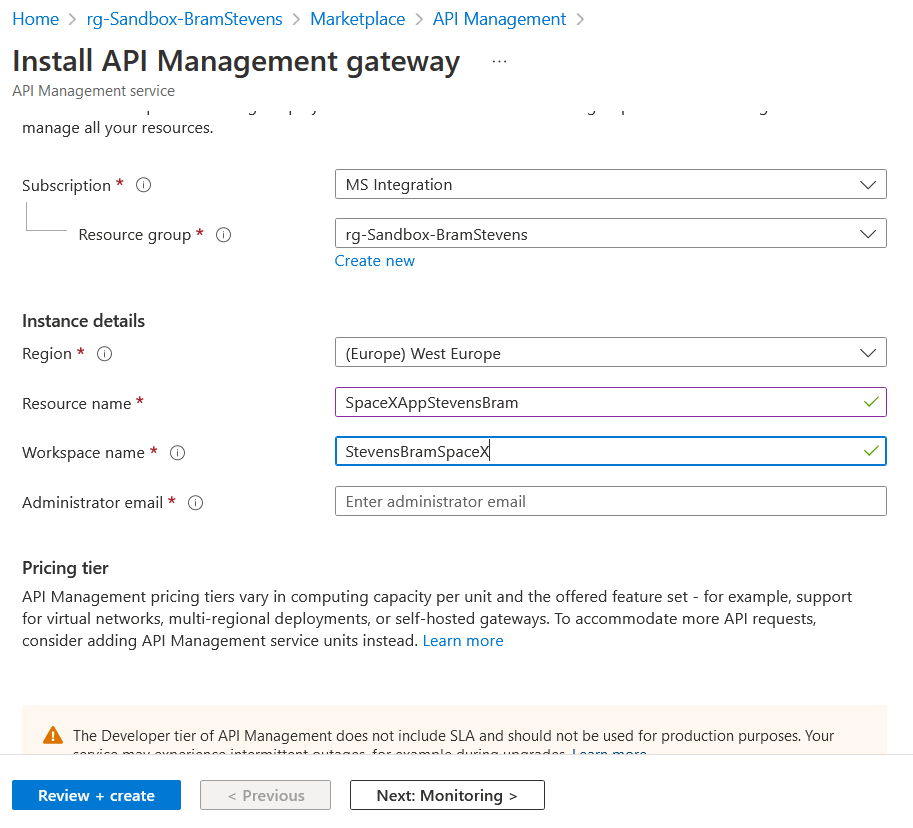
\includegraphics[scale=0.60]{../img/APIManagement.png}
    \caption{\label{fig:APIM}API Management config}
\end{figure}

\begin{figure}
    \centering
    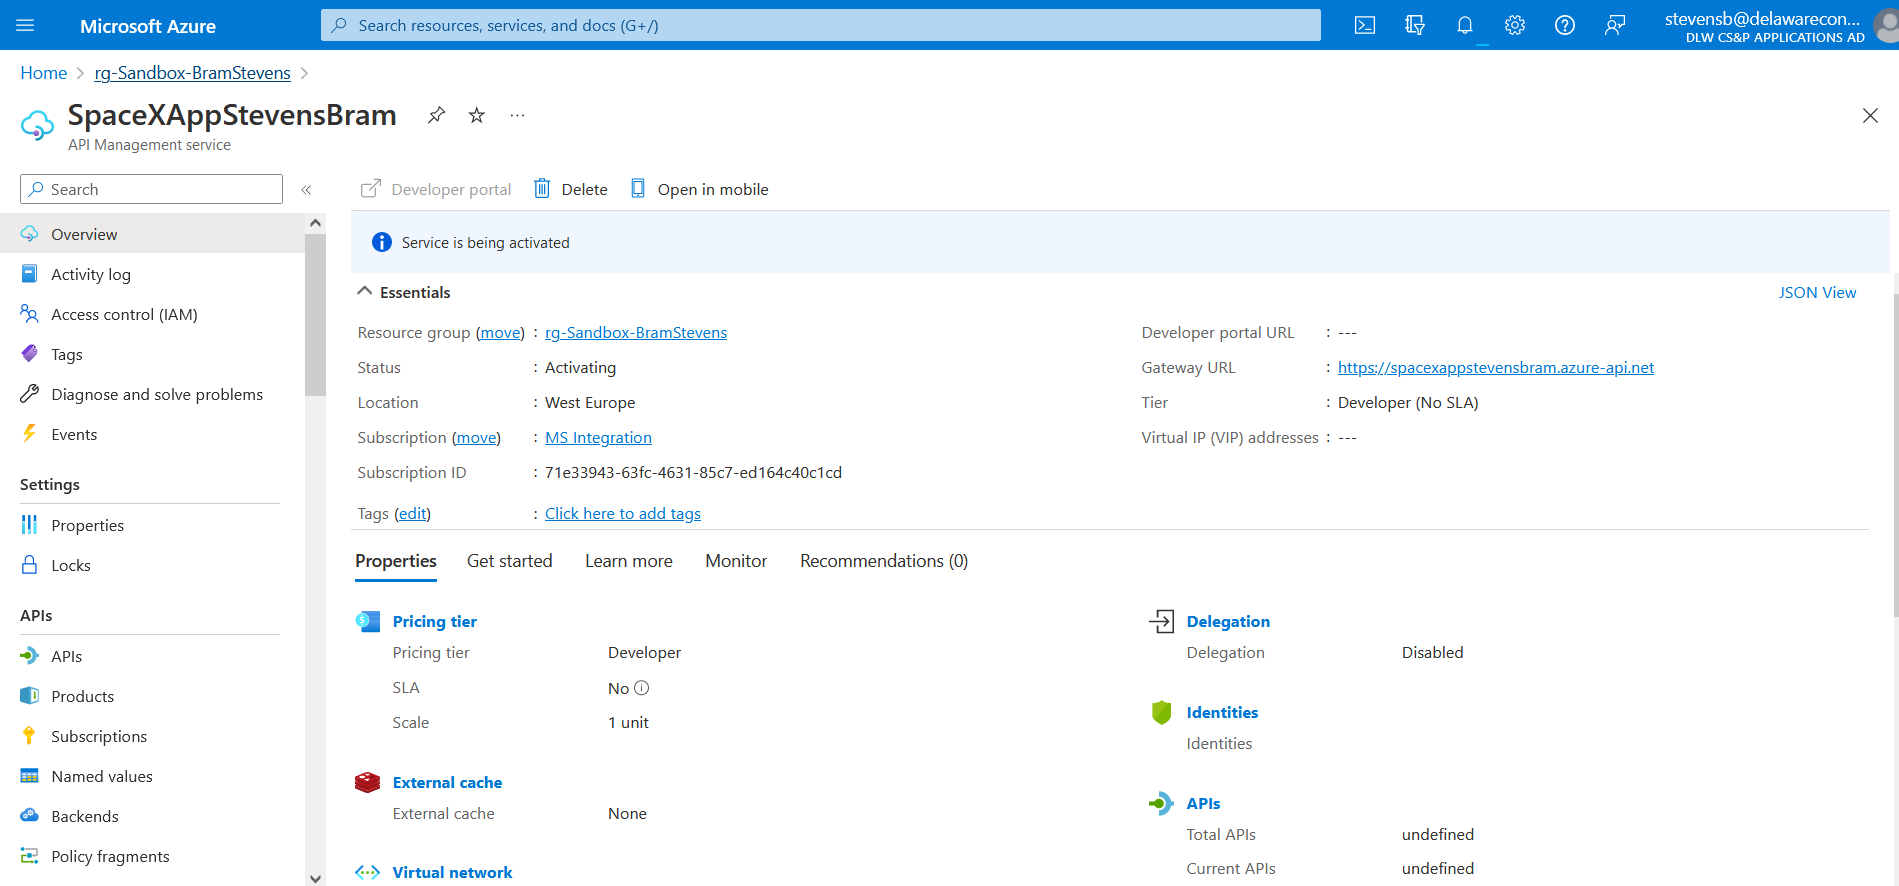
\includegraphics[scale=0.60]{../img/APIService.png}
    \caption{\label{fig:APIS}API Service overview}
\end{figure}

Vervolgens importeert men de benodigde API via de optie in de linker kolom genaamd APIs. In dit menu kan men ook kiezen voor de optie om een nieuwe API aan te maken via de optie Define a new API en de optie GraphQL te selecteren of om een synthetische GraphQL API te creëren en een bijhorend schema bij te voegen. Dit kan ook een gekozen endpoint zijn, Logic of Function App.

Na het creëren van de API kan deze geselecteerd worden en ziet men het scherm dat te vinden is in Figuur~\ref{fig:API}. Hier kan men policies toevoegen en de API testen. Dit gebeurd via de Add inbound policy en te selecteren welke toepassing er benodigt is. Dit bevat onder andere het filtreren van IP adressen en limitaties toevoegen ten opzichte van het aantal requests die tot de backend geraken. Deze kunnen ook verder gepersonaliseerd worden door XML code.

\begin{figure}
    \centering
    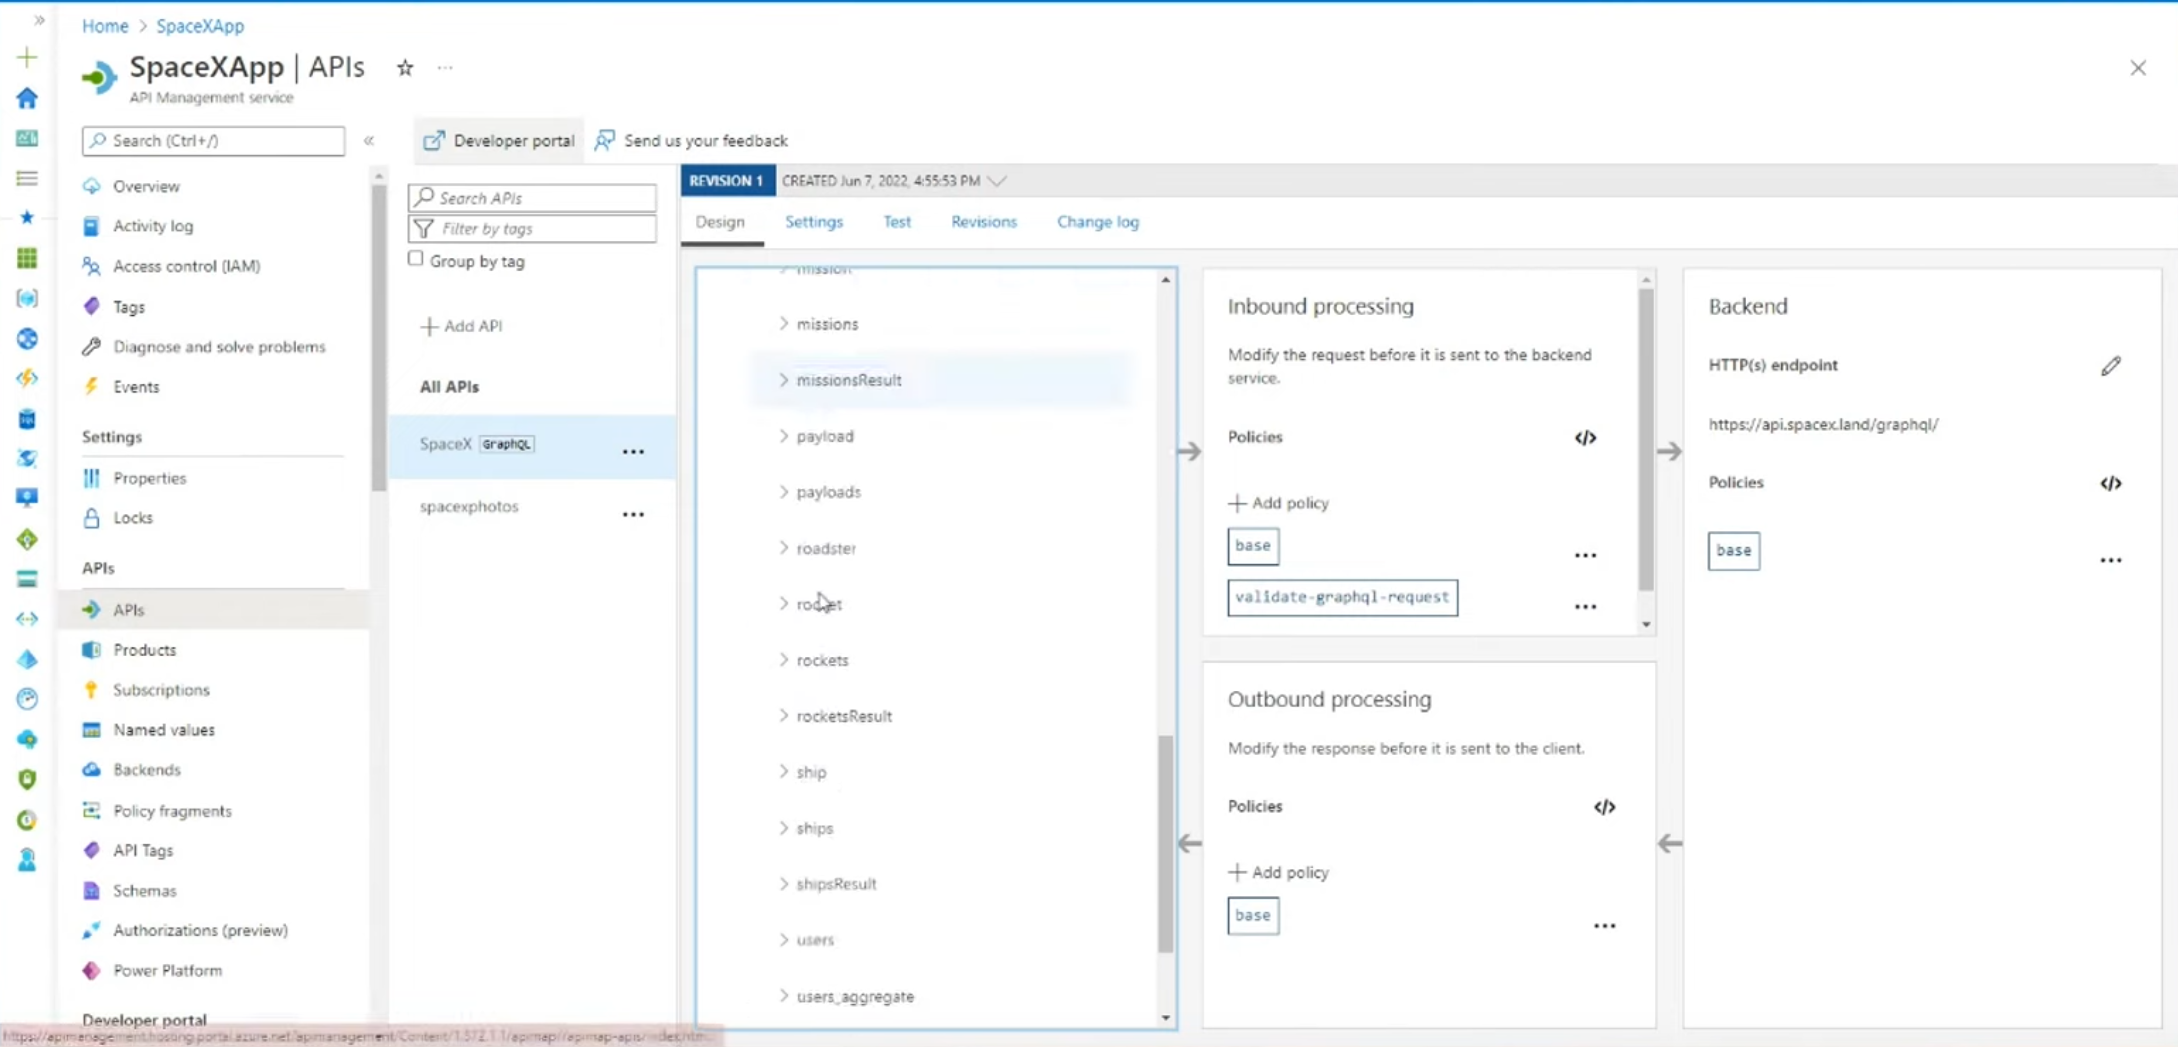
\includegraphics[scale=0.60]{../img/API.png}
    \caption{\label{fig:API}API overview}
\end{figure}

Op voorgaand uitgelegde manier kan men dus eenvoudig GraphQL functionaliteit toevoegen aan een opgestelde omgeving binnen Azure en meteen gebruiken in samenhang met een Data-Accelerator omgeving. Zo is ook de laatste deelvraag beantwoordt: "Kan een Data-Accelerator GraphQL benutten?" Eenmaal de omgeving opgesteld is via de pipeline kan men op slechts enkele minuten tijd GraphQL ondersteuning toevoegen aan de gewenste data zijnde Logic en Function Apps of een endpoint van een bestaande API.

%% TODO: Hoe ben je te werk gegaan? Verdeel je onderzoek in grote fasen, en
%% licht in elke fase toe welke stappen je gevolgd hebt. Verantwoord waarom je
%% op deze manier te werk gegaan bent. Je moet kunnen aantonen dat je de best
%% mogelijke manier toegepast hebt om een antwoord te vinden op de
%% onderzoeksvraag.





% Voeg hier je eigen hoofdstukken toe die de ``corpus'' van je bachelorproef
% vormen. De structuur en titels hangen af van je eigen onderzoek. Je kan bv.
% elke fase in je onderzoek in een apart hoofdstuk bespreken.

%\input{...}
%\input{...}
%...

%%=============================================================================
%% Conclusie
%%=============================================================================

\chapter{Conclusie}%
\label{ch:conclusie}

% TODO: Trek een duidelijke conclusie, in de vorm van een antwoord op de
% onderzoeksvra(a)g(en). Wat was jouw bijdrage aan het onderzoeksdomein en
% hoe biedt dit meerwaarde aan het vakgebied/doelgroep?
% Reflecteer kritisch over het resultaat. In Engelse teksten wordt deze sectie
% ``Discussion'' genoemd. Had je deze uitkomst verwacht? Zijn er zaken die nog
% niet duidelijk zijn?
% Heeft het onderzoek geleid tot nieuwe vragen die uitnodigen tot verder
%onderzoek?





%---------- Bijlagen -----------------------------------------------------------

\appendix

\chapter{Onderzoeksvoorstel}

Het onderwerp van deze bachelorproef is gebaseerd op een onderzoeksvoorstel dat vooraf werd beoordeeld door de promotor. Dat voorstel is opgenomen in deze bijlage.

%% TODO:
%\section*{Samenvatting}

% Kopieer en plak hier de samenvatting (abstract) van je onderzoeksvoorstel.

% Verwijzing naar het bestand met de inhoud van het onderzoeksvoorstel
%---------- Inleiding ---------------------------------------------------------

\section{Introductie}%
\label{sec:introductie}

Meta, voormalig gekend als facebook, ontwikkelde in 2012 een query computertaal genaamd GraphQL om een intern probleem op te lossen. Deze werd in 2015 publiek gesteld en nam sindsdien enorm aan populariteit toe. Veel gekende bedrijven zoals Airbnb, Audi, GitHub, KLM, NBC, PayPal en nog vele anderen gebruiken de computertaal ondertussen al. Ook bij Delaware groeit nu de interesse om zich te verdiepen in GraphQL en de toepassingen die deze technologie met zich meedraagt, rekeninghoudend of dit voor hun een opportuniteit biedt om hun software te verbeteren. In het onderzoek zal dan ook aan bod komen wat die opportuniteiten juist inhouden. Delaware ontwikkelde zelf ook een accelerator die als benaming “Data Accelerator“ kreeg. Wat deze exact doet zal verder uitgelegd worden in sectie 2 - Literatuurstudie.

Vanwege de mogelijke voordelen die een implementatie of integratie van GraphQL met de Data Accelerator kan bieden, wordt dit dus ook het grondthema van deze bachelorproef. Dit op zijn beurt zal theoretisch benaderd worden met als doel naar verloop een fysiek resultaat op te leveren. Deze opzet kan beschreven worden met de volgende onderzoeksvraag: ''Hoe kan GraphQL geïmplementeerd worden in een zelfontwikkelde accelerator?''

Het oogmerk van dit onderzoek is reeds beschreven in de onderzoeksvraag. Echter om deze te behalen moeten de volgende deelvragen beantwoord geraken: \newline - Wat is GraphQL?\newline - Wat is een (Data) Accelerator?\newline - Kan Data Accelerator GraphQL benutten?\newline - Welke integratie mogelijkheden zijn er voor GraphQL binnen Data Accelerator?

Het mikpunt van dit onderzoek is om zo snel mogelijk een concreet voorbeeld te kunnen bieden. Dit is zichtbaar aan de volgorde van de hierbovenstaande deelvragen die opgelijst zijn.


%---------- Stand van zaken ---------------------------------------------------

\section{Literatuurstudie}%
\label{sec:Literatuurstudie}

\subsection{Wat is GraphQL?}
Graph Query Language beter gekend als GraphQL is een query computertaal. Deze maakt gebruik van een API om niet zelf rechtstreeks de data te behandelen. GraphQL brengt een zelfde resultaat tot stand als soortgelijke software, maar op een verschillende manier. Namelijk, de aanvragen worden anders opgebouwd zodat juist de benodigde data ter beschikking komt. De computertaal werd ontwikkeld in 2012 door facebook uit noodzaak tijdens hun converteren naar hun native apps, voorheen mobile apps,
in dienst van hun mobiele website. Soortgelijke software kon hun vereisten niet voldoen vanwege de grote disproportie tussende data en de hoeveelheid server queries die nodig waren. Facebook zocht naar een manier om queries die serverdata collecteren gelijkend te maken aan de samenstelling van hun data. Op deze manier kon er gerichter gewerkt worden om juist de benodigde data ter beschikking te stellen \autocite{Brysbaert2021}.

\subsection{(Data) Accelerator}
Accelerators kunnen gedefinieerd worden als een inhoud bevattende verzameling die inspelen op een vaak voorkomend probleem rondom data kwaliteit. Dit zal vaak in functie van een geografisch gebied of een type van industrie zijn. Deze kan aan de hand van herbruikbare objecten of gespecifieerde regels data analyseren en uitbreiden binnenin een bedrijf. Mogelijks kan deze ook over data domeinen beschikken om verschillende types van info die de data bevat te ontdekken\newline\autocite{Informatica2021}.

Binnenin het computerlandschap zijn er vaak transities van homogene naar heterogene knooppunten. Dit wil zeggen dat in plaats van eenzelfde functie deze gecategoriseerd worden naar gelang hun functie. Dit kan u best vergelijken met het verschil tussen een koper en een verkoper van schoenen. Accelerators kunnen in functie staan van een grafische processor, computerchips die over meerdere kernen beschikken, schakelingen van logische componenten of een microprocessor om digitale signalen te bewerken. Hier is hun doel dan om taken die heel reken-intensief zijn, te lichten voor het systeem \autocite{LopezNovoa2015}.

De accelerator die in gebruik gesteld wordt van Delaware in functie van dit onderzoek zal verder uitgespit worden in deze bachelorproef zodat er een duidelijk gedefinieerde basis is waaruit er vertrokken wordt.

%---------- Methodologie ------------------------------------------------------
\section{Methodologie}%
\label{sec:methodologie}

Om de opgelijste deelvragen te kunnen beantwoorden is er een literatuurstudie nodig als startpunt. Daarom is dit dus ook de eerste fase van het onderzoek. In de literatuurstudie kan het volgende nagekeken worden:\newline Wat is de exacte werking van GraphQL en hoe implementeerd of integreert men dit?\newline Welke opportuniteiten of nadelen kan GraphQL opleveren?\newline Kan men GraphQL integreren in een accelerator of moet men implementeren? \newline Wat is de complexiteit van de uit te voeren integratie of implementatie?

Hiervoor wordt er een case study uitgevoerd die kan nagaan welke oplossing juist het meest voordelig is en of Microsoft Azure al dan niet soortgelijke implementaties reeds bevat. Zo kunnen we nagaan of deze implementatie nodig is of op een andere manier bereikt kan worden.

%---------- Verwachte resultaten ----------------------------------------------
\section{Verwachte resultaat}
\label{sec:verwachte resultaat}
Het verwachte resultaat van deze case study moet een praktische oplossing zijn voor de implementatie van GraphQL. Dit moet een overzicht kunnen leveren aan lezers die zich willen verdiepen in deze kwestie. Voor Delaware moet het mogelijk zijn om evenals een duidelijk stappenplan te verkrijgen om dit dan effectief ook uit te voeren indien gewenst. De mogelijke alternatieve oplossingen binnen Azure zouden hier dan ook aangekaart worden.

\section{Verwachte conclusie}
\label{sec:verwachte conclusiet}
Als echter vele bedrijven reeds de stap zetten en gebruikmaken van GraphQL is dit voor Delaware ook interessant om te zien welke mogelijke toepassingen er allemaal zijn die in hun voordeel spelen. Er is een grote kans dat het mogelijk is om GraphQL en Data Accelerator samen te laten werken via integratie of implementatie. Evenals is het niet ondenkbaar dat Microsoft Azure functies bevat waarvoor het onnodig kan zijn wegens betere alternatieven.


\chapter{bijlagen}

\section{Workflow}%
\label{sec:Workflow}
\begin{figure}[H]
    \centering
    \includegraphics[]{img/Workflow.PNG}
\end{figure}




%%---------- Andere bijlagen --------------------------------------------------
% TODO: Voeg hier eventuele andere bijlagen toe. Bv. als je deze BP voor de
% tweede keer indient, een overzicht van de verbeteringen t.o.v. het origineel.
%\input{...}
\chapter{Bijlagen}
\section{main.template.bicep}
\label{sec:main.template.bicep}
\begin{lstlisting}
    // main.template.bicep
    //* --- PARAMETERS ---
    @description('Name of the environment to deploy the resources to')
    param dIPEnvironment string
    param dIPCompany string
    param dIPLocation string = resourceGroup().location
    param dIPName string
    param KeyvaultName string
    param UserAssignedIdentityName string
    param adminName string
    param adminPW string
    param usePE bool
    param vNet string
    param privateDnsZoneBlob string
    param privateDnsZoneQueue string
    param privateDnsZoneWeb string

    //* --- MODULES ---
    module dIP_Framework 'Framework/_framework.template.bicep'  = {
        name: 'dip-framework'
        params: {
            dIPEnvironment: dIPEnvironment
            dIPCompany: dIPCompany
            dIPLocation: dIPLocation
            dIPName: dIPName
            KeyVaultName: KeyvaultName
            UserAssignedIdentityName: UserAssignedIdentityName
            adminName: adminName
            adminPW: adminPW
            usePE: usePE
            vNet: vNet
            privateDnsZoneBlob: privateDnsZoneBlob
            privateDnsZoneQueue: privateDnsZoneQueue
            privateDnsZoneWeb: privateDnsZoneWeb
        }
    }

\end{lstlisting}
%%---------- Backmatter, referentielijst ---------------------------------------

\backmatter{}

\setlength\bibitemsep{2pt} %% Add Some space between the bibliograpy entries
\printbibliography[heading=bibintoc]

\end{document}
